\documentclass[t]{beamer}

\usetheme{CambridgeUS}
\usecolortheme{beaver}
\setbeamertemplate{navigation symbols}{}

\usepackage[utf8]{inputenc}
\usepackage[croatian]{babel}

\usepackage{datetime}
\renewcommand{\dateseparator}{.}
\newcommand{\todayiso}{\twodigit\day \dateseparator \twodigit\month \dateseparator \the \year}
\date{\todayiso}

\usepackage{listing}
\usepackage{graphicx}
\usepackage{subcaption}
\captionsetup{compatibility=false}


\title[NKOSL]{Napredno korištenje operacijskog sustava Linux}
\author[Dominik Barbarić]{Dominik Barbarić\\{\small Nositelj: Stjepan Groš}}
\subtitle{1. Boot proces i datotečni sustavi}
\institute[FER]{Sveučilište u Zagrebu\\Fakultet elektrotehnike i računarstva}

\begin{document}

{
	\setbeamertemplate{footline}{}
	\begin{frame}
		\maketitle
	\end{frame}
}

\begin{frame}
	\frametitle{Sadržaj}
	\tableofcontents
\end{frame}

\section{BIOS}
\begin{frame}
	\frametitle{BIOS}
	\textbf{B}asic \textbf{I}nput and \textbf{O}utput \textbf{S}ystem
	\begin{itemize}
		\item Firmware na matičnoj ploči
		\item Pokreće se na startupu
		\item Izvršava Power-on self-test (POST) nad matičnom i drugim spojenim uređajima (S.M.A.R.T. test diskova, Extension ROM dodatnih uređaja itd.)
		\item Konfigurira se preko ugrađenog firmwarea ili hardverski (jumperi, DIP switchevi, ... )
		\item Omogućuje odabir uređaja s kojeg se pokreće operacijski sustav
	\end{itemize}
\end{frame}

\begin{frame}
	\frametitle{Particije}
	\begin{itemize}
		\item Hard disk sadrži particije formatirane određenim datotečnim sustavom
		\item Informacije o particijama sadržane u
		\begin{itemize}
			\item Master boot record (MBR)
			\item GUID Partition Table (GPT)
		\end{itemize}
	\end{itemize}
\end{frame}	

\begin{frame}
	\frametitle{MBR}
	\begin{itemize}
		\item Zapisan u prvom sektoru diska (512 B / 2 KiB)
		\begin{itemize}
			\item Partition table
			\item \textbf{Bootstrap code} - minimalni podaci potrebni za nastavak boot procesa
			\item ...
		\end{itemize}
		\item Podržava 4 \emph{primarne} particije
		\item Za veći broj particija koriste se \emph{logičke} particije koje se upisuju u jednu primarnu particiju tipa \emph{extended}
	\end{itemize}
\end{frame}

\begin{frame}
	\frametitle{GPT}
	\begin{itemize}
		\item Dio UEFI standarda
		\item Podržava velike diskove 
		\item Proizvoljan broj particija
	\end{itemize}
	\begin{itemize}
		\item \emph{Protective MBR} - omogućuje kompatibilnost s BIOS sustavima
		\item UEFI sustavi mogu izravno pozivati bootloadere iz particija
	\end{itemize}
\end{frame}

\section{Bootloader}
\begin{frame}
	\frametitle{Bootloader}
	\begin{itemize}
		\item Izvršava se nakon POST
		\item Pokreće operacijski sustav - učitava kernel
	\end{itemize}
	
	\begin{itemize}
		\item Prva faza bootloadera zapisana u bootstrap code MBR diskova
		\item Često se pokreće druga faza s neke od particija
	\end{itemize}
	\begin{itemize}
		\item GPT diskovi
		\begin{itemize}
	 		\item Protective MBR - isto kao i kod MBR diskova
			\item UEFI-GPT boot
		\end{itemize}
	\end{itemize}
\end{frame}

\begin{frame}
	\frametitle{Bootloderi}
	\textbf{GR}and \textbf{U}nified \textbf{B}ootloader
	\begin{itemize}
		\item GNU projekt
		\item Konfigurabilan za više operacijskih sustava na jednom računalu
	\end{itemize}
	\begin{itemize}
		\item \textbf{GRUB Legacy}
		\begin{itemize}
			\item Starija verzija
			\item Više se ne razvija
		\end{itemize}
		\item \textbf{GRUB 2}
		\begin{itemize}
			\item Drugačije konfiguracijske datoteke
			\item Modularan, puno mogućnosti
			\item Zauzima puno više prostora od GRUB Legacy
		\end{itemize}
	\end{itemize}
	\vfill
	Syslinux
	\begin{itemize}
		\item \emph{Lightweight} bootloader
		\item Jednostavna konfiguracija
	\end{itemize}
\end{frame}

\begin{frame}
	\frametitle{Druge platforme}
	Linux pokreće bootloader ili firmware
	\begin{figure}
		\centering
		\begin{subfigure}[f]{0.55\textwidth}
			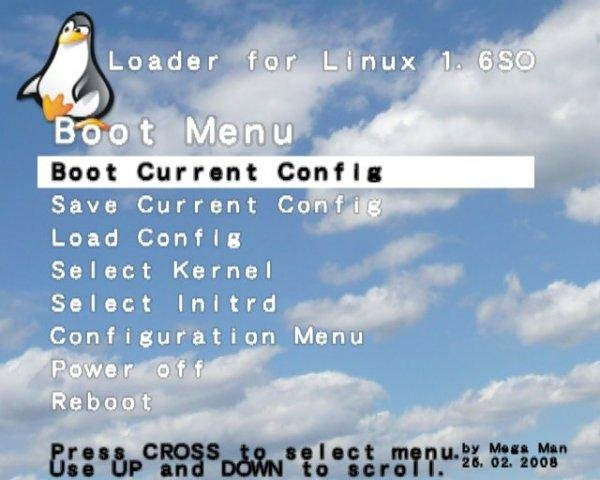
\includegraphics[width=\textwidth]{ps2kernelloader.jpg}
			\caption*{Play Station 2 \emph{kernelloader}}
		\end{subfigure}
		\hfill
		\begin{subfigure}[f]{0.3\textwidth}
			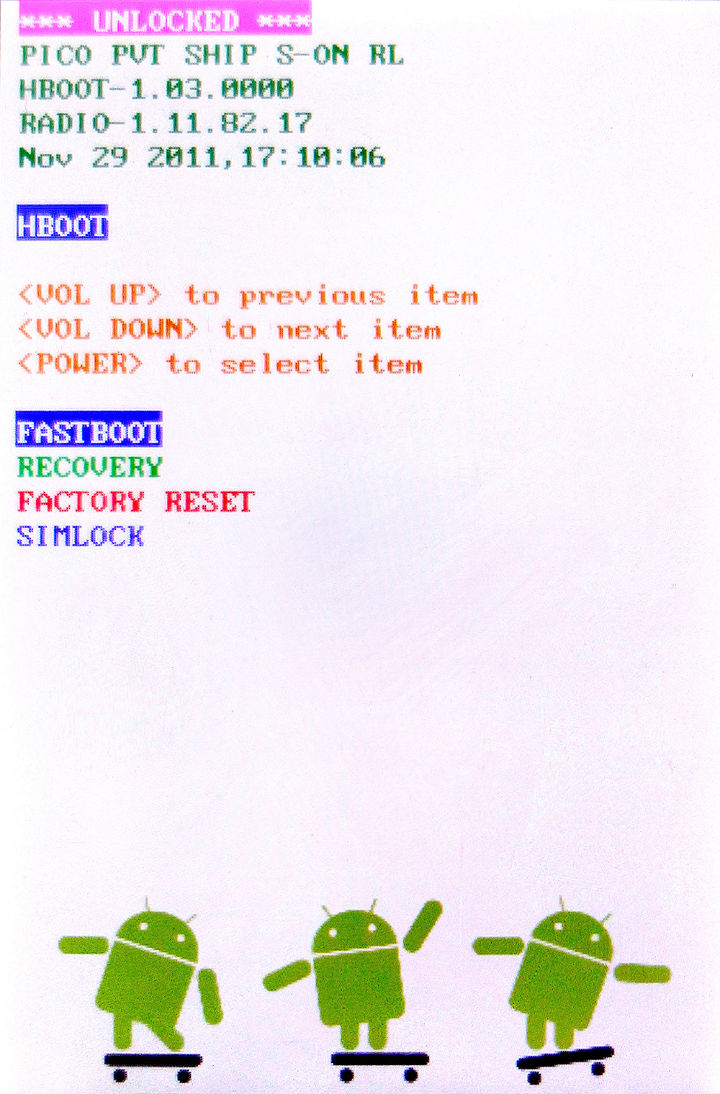
\includegraphics[width=\textwidth]{androidHboot.jpg}
			\caption*{HTC Android Hboot}
		\end{subfigure}
	\end{figure}
\end{frame}

\begin{frame}
	\frametitle{initrd / initramfs}
	\begin{itemize}
		\item Kernel prepoznaje sve uređaje na sustavu i učitava
		\item[] \emph{initial ramdisk}
		\item[]
		\item Omogućuje kernelu učitavanje osnovnih modula kako bi došao do \emph{root} filesystema
		\begin{itemize}
			\item moduli
			\item enkripcija
			\item RAID / LVM
			\item \dots
		\end{itemize}
		\item[]
		\item initrd se po završetku briše iz memorije
		\item Pokreće se init
	\end{itemize}
\end{frame}

\section{init, systemd}
\begin{frame}
	\frametitle{init}
	\begin{itemize}
		\item System V uvodi koncept \emph{runlevel}-a
	\end{itemize}
	\begin{itemize}
		\item U Linuxu definirano nekoliko runlevel-a
		\begin{description}
			\item[0] - Sustav se isključuje
			\item[1 / S] - Single user mode
			\item[2 - 5] - Multi user mode (ili nešto drugo)
			\item[6] - Ponovno pokretanje
		\end{description}
		\item Stvarni \textit{startup} level je određen u datoteci \texttt{/etc/inittab}
	\end{itemize}
\end{frame}

\begin{frame}
	\frametitle{init}
	\begin{itemize}
		\item Kod ulaska u svaki runlevel pokreću se skripte
		\item[] \texttt{/etc/rc.d/rc?.d}
		\item[]
		\item Poredak izvođenja skripti je određen imenom skripte u folderu:
		\begin{itemize}
			\item[] \textbf{K01-K99} - skripta gasi servis pri ulasku u runlevel
			\item[] \textbf{S01-S99} - skripta pokreće servis pri ulasku u runlevel
		\end{itemize}
		\item Nakon izvođenja svih skripti u folderu pokreće se i \texttt{/etc/rc.local}
		\item[]
	\end{itemize}
	Sve što se nalazi u direktorijima \texttt{/etc/rc.d} je obično samo symlink na skripte u \texttt{/etc/init.d}
\end{frame}

\begin{frame}
	\frametitle{systemd}
	\begin{itemize}
		\item Zamjenjuje init na sve više distribucija
		\item Sustav upravljanja procesima i cijelim sustavom
	\end{itemize}
	\begin{itemize}
		\item Konfiguracija zasnovana na \emph{unit} datotekama
		\item Neki tipovi \emph{unit} datoteka
		\begin{description}
			\item[service] opisuje servis na sustavu
			\item[target] grupira unit-e u skupine
			\item[\dots]
		\end{description}
	\end{itemize}
	\vfill
	\texttt{systemctl} \\ \texttt{journalctl}
\end{frame}

\section*{}
\begin{frame}
	\frametitle{Literatura}
	\url{http://en.wikipedia.org/wiki/Comparison_of_file_systems}\\
	\url{http://www.pathname.com/fhs/}\\
	\vfill
	\url{https://wiki.archlinux.org/index.php/GRUB_Legacy}\\
	\url{https://wiki.archlinux.org/index.php/GRUB}\\
	\url{http://wiki.gentoo.org/wiki/GRUB2_Quick_Start}\\
	\vfill
	\url{http://users.cecs.anu.edu.au/~okeefe/p2b/power2bash/power2bash.html}\\
\end{frame}

\end{document}
